{\let\clearpage\relax\let\cleardoublepage\relax
\chapter{Simulazione popolazioni planetarie}
}

\begin{workout}[Ref PPS]
Towarddeterminist model of planetary formation iV: effectsof type I migration
									: accumulation neare iceline
									: dynamical intaraction and coagulation of multiple rocky embrios (isolation mass, semi-analytic vs n-body)
									: eccentricity distribution of gas giant
\end{workout}

\section{Modello disco di accrescimento e distribuzione condizioni iniziali}

\begin{workout}[Modello di disco di accrescimento - (Mordasini18: 4) - Introduzione descrizione fenomeni grazie a PPS]
Refs: garaud lin 07, chiang goldreich 97
Un modello di disco  di accrescimento usato nelle simulazioni considera l'evoluzione della densit\'a superficiale tramite l'equazione \eqref{eq:diskaccrphev-m18}

\begin{align}
&\TDy{t}{\Sigma}=\frac{1}{r}\PDof{r}[3r\expy{1/2}\PDof{r}(\nu\Sigma r\expy{1/2})]+\dot{\Sigma}_w(r)+\dot{\Sigma}_p(r)\label{eq:diskaccrphev-m18}\\
&\dot{\Sigma}_w(a)=\left\{\begin{array}{c}0\\\frac{\dot{M}_w}{2\pi(a_{max}-R_g)a}\\\end{array}\right.
\end{align}

Densit\'a superficiale iniziale:
\begin{equation}
\Sigma(a,t=0)=\Sigma_0(\frac{r}{1AU})\expy{p_g}\Exp{[-(\frac{r}{R_o})\expy{2+p_g}]}(1-\sqrt{\frac{r}{R_i}})
\end{equation}
4-Mordasini18 (Hayashi81). $p_g\approx1$ (Andrews10).
\end{workout}

Initial disk mass
(infall phase end, no more self-gravitational instabilities) - stability(shu90), MMSN hayashi81/weidenshilling77, observations(Andrews10,Manara16) points to $(0.1-10)\%$ stellar mass, distro log-normal with mean $0.01M_*$.

{Disk lifetime}
$1-10My$ with mean $3My$ (Haisch01, Mamajek09)


\section{Distribuzione iniziale planetesimi}
Assumendo conversione completa di polvere in planetesimi, la densit\'a superficiale di planetesimi \'e
\begin{equation}
\Sigma_p(t=0,r)=f_{dg}\eta_{ice}\Sigma_g(t=0,r)
\end{equation}

\begin{workout}[Initial planetesimal distro]
Dust converted early everywhere fully-efficient (mordasini18: pg 12),Thommes pg8)
\begin{align*}
&\Sigma_p(t=0,r)=f_{dg}\eta_{ice}\Sigma_g(t=0,r)\\
&\dot{\Sigma}_p(r)=-\frac{1}{2\pi aB_LR_H}\dot{M}_c
\end{align*}
Icelines Mordasini 1141: inside where T exceeds sublimation

{Embryo starting position}
Usually a distro uniform in log(a): relative spacing of few Hill spheres (Kokubo Ida 10)
Ida, lin10: asymptotical isolation mass ''Toward a Deterministic Model of Planetary Formation VI'',
Trapped evolution model: Hasegawa pudritz 11, Cridland 16

\end{workout}

\section{Accrescimento dei protopianeti e gas}

La massa dei core varia secondo
\begin{align}
&\dot{M}_c=\Omega\Sigma_pR^2_{capt}F_G\\
&\dot{\Sigma}_p(r)=-\frac{1}{2\pi aB_LR_H}\dot{M}_c
\end{align}

Si risolvono numericamente le equazioni di conservazione di massa, equilibrio idrostatico, conservazione/trasporto energia 1D

\begin{workout}[Attached phase: boundary conditions]
\begin{align}
&P_{pl}=P_{Neb}\\
&T_{Pl}=T_{Neb}\\
&R_{Pl}=Min(R_H,R_H)
\end{align}
\end{workout}


\begin{workout}[Detached phase: transition condition and boundary condition]
Transition attached/detched phase $\approx10\mearth{}$.
Accretion shock for free-falling materials from Hill radius (more realistic circumplanetary disk: Papailoizou Nelson 05)
\begin{align}
&\dot{M}_{XY}^{max}\\
&v_{ff}^2=2GM(\frac{1}{R}-\frac{1}{R_H})\\
&P=P_{neb}+\frac{\dot{M}_{XY}}{4\pi R^2}v_{ff}+\frac{2g}{3\kappa}\\
&\tau=max(\rho_{neb}\kappa_{neb}R,2/3)\\
&T^4_{int}=\frac{3\tau L_{int}}{8\pi\sigma R^2},\ T^4=(1-A)T_{neb}^4+T_{int}^4
\end{align}
$R\approx1.5-5\rjupiter{}$ depending on entropy: THE PLANETARY ACCRETION SHOCK:I. FRAMEWORK FOR RADIATION-HYDRODYNAMICAL SIMULATIONS AND FIRST RESULTS (m17), Characterization of exoplanets from their formation III: The statistics of planetary luminosities (m17)
Bondi accretion rate: $\dot{M}_{e, Bondi}\approx\frac{\Sigma}{H}(R_H/3)^3\Omega$ or viscous accretion rate $\dot{M}_{e, visc}\approx f_{lub}3\pi\nu\Sigma_g$
\end{workout}

\begin{workout}[Higher mass gap formation reduces accretion rate]
\begin{equation}
f_{va04}=1.668(\frac{M_p}{\mjupiter{}})\expy{1/3}\exp{-\frac{M_p}{1.5\mjupiter{}}}+0.04
\end{equation}
\end{workout}

\section{Popolazione sintetiche}

%envelopcore
\begin{figure}
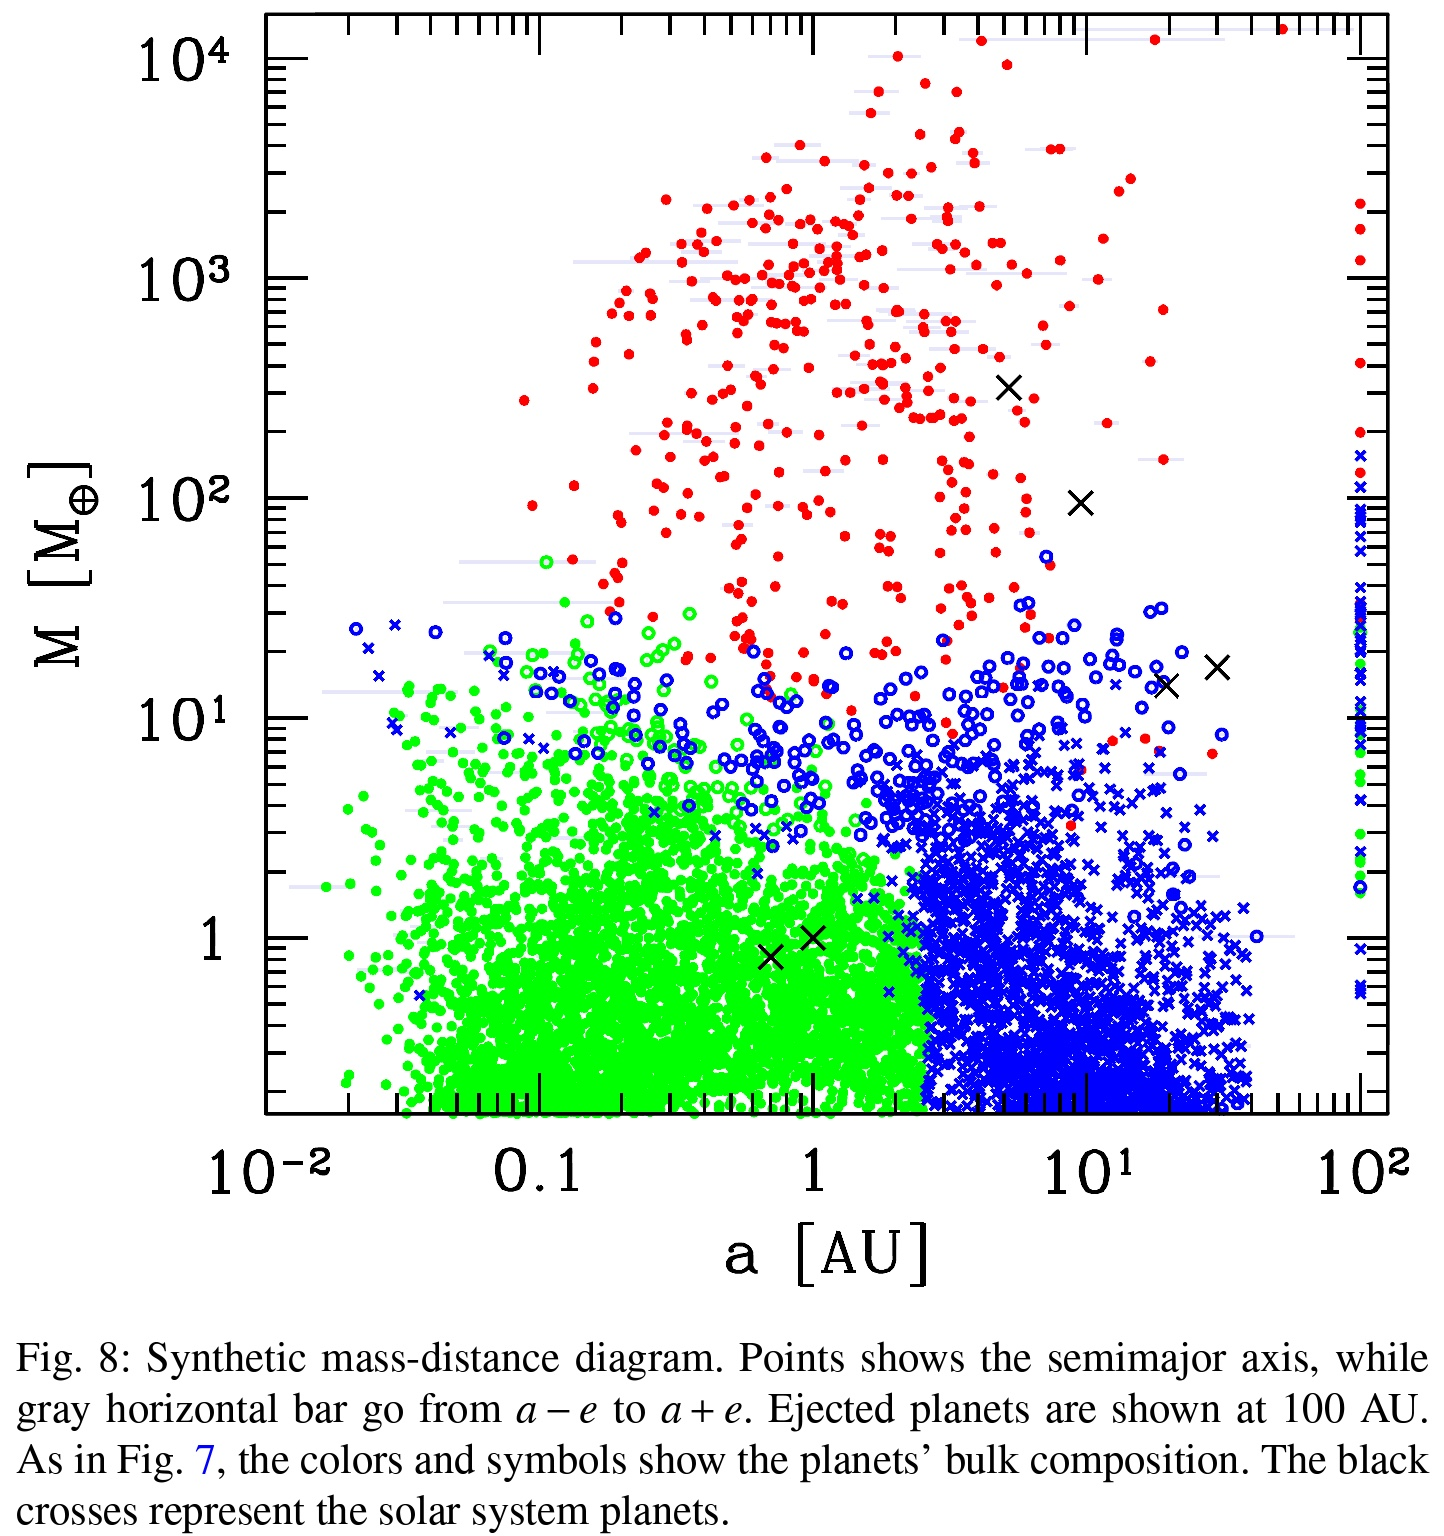
\includegraphics[]{ma-synth}
\caption{Punti rossi: pianeti giganti con $M_e/M_c>1$; blu have accreted ices outside iceline while green have accreted solidi refrattarii}
\end{figure}

{\let\clearpage\relax\let\cleardoublepage\relax
\chapter{Raffronto popolazione osservata vs sintetiche}
}

\begin{workout}[Effects of saturation, cooling and irradiation.]
Impact of planet migration model on planetary populations: effects of saturation, cooling and stellar irradiation (??)
Outward migration helps some planets to become massive, accumulation zone at certain semiaxis, at what mass corotation saturate?
Migration of protoplanets in radiative disks
\end{workout}
